\documentclass[11pt]{article}
\usepackage[utf8]{inputenc}
\usepackage[english]{babel}
\usepackage{graphicx}
\usepackage[numbers]{natbib}

\graphicspath{{pics/}}


\title{KRKPA7 problem in various data mining software \\ 4IZ451 - Knowledge discovery in databases}
\author{Tomáš Maršálek}
\date{\today}

\begin{document}
\maketitle
\thispagestyle{empty}
\clearpage

\section{Introduction}
The purpose of this work is to analyze database of KRKPA7 problem using four different data mining tools. Some of the chosen data mining programs are freely available (Weka) or freely available for non-commercial use (RapidMiner) or proprietary licensed (Enterprise Modeler, IBM PASW). %% TODO je to tak do řitě?
The nature of problem for this assignment is suitable for classification and association modeling, but not for clustering.

\section{KRKPA7 problem}
KRKPA7 is a shorthand for King Rook versus King Pawn on A7, which is a chess endgame. The black player has a king and a pawn left, where the pawn is on A7, which is one turn away from turning his into a queen. The white player has a turn in this situation and has a king and a rook to play with.

\begin{figure}[!ht]
	\centering
	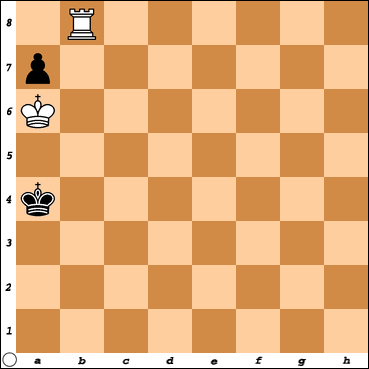
\includegraphics[width=.7\textwidth]{example}
	\caption{Example board set up}
\end{figure}

\clearpage

\subsection{Data set}
Data set contains 3196 set ups of chess board, each one with different positions of both kings and the rook, the pawn is fixed on A7.

Each board set up is described by 36 attributes described in table \ref{tab:attributes}.

\section{Weka}
\section{IBM PASW}
\section{Enterprise Modeler}
\section{Rapid Miner}


\begin{table}[h]
\makebox[\textwidth][c]{
\begin{tabular}{|l|l|l|}
\hline
position & shorthand & description \\
\hline
1	&bkblk	&the BK is not in the way \\
2	&bknwy	&the BK is not in the BR's way \\
3	&bkon8	&the BK is on rank 8 in a position to aid the BR \\
4	&bkona	&the BK is on file A in a position to aid the BR \\
5	&bkspr	&the BK can support the BR \\
6	&bkxbq	&the BK is not attacked in some way by the pro- moted WP \\
7	&bkxcr	&the BK can attack the critical square (b7) \\
8	&bkxwp	&the BK can attack the WP \\
9	&blxwp	&B attacks the WP (BR in direction x = -1 only) \\
10	&bxqsq	&one or more Black pieces control the queening square \\
11	&cntxt	&the WK is on an edge and not on a8 \\
12	&dsopp	&the kings are in normal opposition \\
13	&dwipd	&the WK distance to intersect point is too great \\
14	&hdchk	&there is a good delay because there is a hidden check \\
15	&katri	&the BK controls the intersect point \\
16	&mulch	&B can renew the check to good advantage \\
17	&qxmsq	&the mating square is attacked in some way by the promoted WP \\
18	&r2ar8	&the BR does not have safe access to file A or rank 8 \\
19	&reskd	&the WK can be reskewered via a delayed skewer \\
20	&reskr	&the BR alone can renew the skewer threat \\
21	&rimmx	&the BR can be captured safely \\
22	&rkxwp	&the BR bears on the WP (direction x = -1 only) \\
23	&rxmsq	&the BR attacks a mating square safely \\
24	&simpl	&a very simple pattern applies \\
25	&skach	&the WK can be skewered after one or more checks \\
26	&skewr	&there is a potential skewer as opposed to fork \\
27	&skrxp	&the BR can achieve a skewer or the BK attacks the WP \\
28	&spcop	&there is a special opposition pattern present \\
29	&stlmt	&the WK is in stalemate \\
30	&thrsk	&there is a skewer threat lurking \\
31	&wkcti	&the WK cannot control the intersect point \\
32	&wkna8	&the WK is on square a8 \\
33	&wknck	&the WK is in check \\
34	&wkovl	&the WK is overloaded \\
35	&wkpos	&the WK is in a potential skewer position \\
36	&wtoeg	&the WK is one away from the relevant edge \\
\hline
\end{tabular}
}
\caption{Board positions attributes~\citep{Michie1995-MICCAA-2}}
\label{tab:attributes}
\end{table}

\clearpage
\bibliographystyle{csplainnat}
\bibliography{ref}

\end{document}
